\documentclass[11pt]{article}

\renewcommand{\rmdefault}{phv} % Arial
\renewcommand{\sfdefault}{phv} % Arial

\usepackage{graphicx}

\oddsidemargin=0in
\textwidth=6.5in
\textheight=9in
\topmargin=-.625in
\linespread{1.4}

\begin{document}
\begin{center}
{\Large \textbf{Collaborative Research: Resource of Open\\
Problems for Education (ROPE)}}
\end{center}

\begin{section}{Introduction}

At the heart of teaching and learning mathematics---and many other
disciplines---is a learner's engagement with questions, or problems, which
challenge her or him to understand and apply the material s/he is
learning.  We propose to develop a resource that will provide an on-line
electronic library of innovative, well-tested and documented problems that
instructors and students may use in a wide range of courses and for a wide
range of assignment types.  This ``Resource of Open Problems for
Education'' (ROPE) will allow searching and browsing to find appropriate
problems; will include descriptive information about problem usage and the
numbers of users endorsing the problems; and will allow users to share
problem collections and lists drawn from the library.  Because it will be
an open resource, institutions and individuals with limited resources will
still have full access to it, and the community of ROPE users will be able
to provide added value to the library.  The motivations for ROPE are:
\begin{itemize}
  \item
    To be a \textit{free, open-source resource} that will give instructors
    and students access to good mathematics problems.  The cost of
    textbooks and supporting materials for courses is increasingly
    untenable.  We believe that as academic practitioners we should work
    to have an accessible resource that does not discriminate on the basis
    of wealth and which does not demand advertising or private data for
    its use.
  \item
    To be an \textit{extensive, broad, and well-vetted resource} of
    problems that can complement existing text problems, be used with
    open-source textbooks, or be used to create practice worksheets,
    quizzes or exams.  Instructors and students benefit from the
    availability of good problems that they may use directly or adapt.
  \item
    To provide the mechanism for a \textit{community of users} of these
    problems, who may contribute problems, content and feedback on
    problems, and who may share the groups of problems they use for
    specific homework sets or courses.
\end{itemize}

\end{section}

\begin{section}{Description}

Internet users go to Amazon to search for material products to buy.  We
hope to develop ROPE into the place where mathematics teachers and
learners go to find problems and inspiration for problems for the courses
they are teaching and learning.



Users will be able to search this library
for problems by course, topic, type of problem (e.g., computational,
conceptual, etc.), level of difficulty, and other characteristics.
Problems will be contributed by the community of users and will have
associated descriptive information that will include user feedback and
comments, as well as statistics on the frequency of the problem's use.
Users will be able to rate problems using a commonly understood ``like''
feature (similar to those used on social networking sites), they will be
able to create and share collections of problems they may refer to later
for use in homework, quizzes or exams, and they will be able to comment on
problems for the benefit of other users.  The problems will be available
in multiple formats, and will be applicable to different uses.  In time we
expect that the library will be extended to include other disciplines
besides mathematics.

This electronic library will be an open library: problems will be openly
available for use and modification by all users.  Open-source software has
a (relatively) long and well-established history and tradition in the
development of modern computing platforms, and provides the basis for a
large portion of the computing infrastructure on which current technology
from the Internet to smartphones run.  The idea underlying this software,
of an open development of resources that may be taken, redeveloped and
repurposed for the common good, is one which these same technologies are
increasingly making available to other venues. We are seeing the
development of open-content textbooks, websites that allow open sharing of
expertise in programming, car repair and evaluation of professorial
instruction, and more.  In this environment a Resource of Open Problems for Education (ROPE) will
not only fit in, but thrive.

It is an opportune time for the development of this resource of open problems.  Mathematics educators are exploring innovative pedagogies
including writing projects, inquiry-based learning, and on-line teaching
and assessment.  There is a substantial community that is developing
open-content textbooks and open-source software as a reaction to high
textbook prices and expensive proprietary educational and research
software.  There are natural connections between the proposed ROPE and
educators who are looking for new resources in their teaching, as well as
with the open-content texts and open-source software that are being
developed.  ROPE will provide pedagogical innovators with new and
different problems to use as they work on different ways to improve their
instruction; will provide authors and users of open-content textbooks a
problem resource to populate and augment the problem lists in their texts;
and will be able to connect with open-source software projects that
deliver and display mathematical content and problems.

As a result of these connections and flexibility, we expect ROPE to be
used by instructors in a wide range of manners.  Instructors will be able
to use it to construct homework sets in courses for which they have
lecture notes but an inadequate set of available homework problems.  They
will be able to use it to augment the problems that they have available
from their textbook, for use on homework sets, quizzes, exams, or other
assignments---a use which may be particularly relevant for users of
open-content texts.  Authors will be able to use it as a resource for
problems and problem sets for their textbooks, and will be able to
contribute problems for their texts to the library.  On-line courses and
homework systems will be able to use it to populate their assignments.  To
provide for its long-term sustainability and flexibility, ROPE will
have an underlying data structure that will allow the addition of new
problem formats and filters to transform existing formats into others
(e.g., by transforming a problem written in \LaTeX\ to HTML or PDF, or
from \LaTeX\ to a problem for an on-line homework system) and include a
well-documented and extensible Application Programming Interface
(API). Through the latter, other applications will be able to ``talk'' to
ROPE; this will allow the library to serve problems to other resources
(e.g., the problem library for an on-line homework system).

\end{section}

\begin{section}{Context}

While there is no resource currently available that provides the
functionality and material that will be included in the Resource of Open
Problems for Education, there is existing software that will provide a basis for ROPE,
and which will inform its development.  Three applications that are closely
related to the work we seek to do with ROPE are: an existing problem
library developed in the mathematics department at the University of
Michigan by Gavin LaRose; the National Problem Library (NPL) used by
the WeBWorK [3] %\cite{webwork} 
on-line testing and assessment system, for
which Gavin LaRose has been a software developer; and Edfinity, a  
proprietary startup providing content and self-publishing options
for educators.

The problem library in use at the University of Michigan currently
provides a subset of the features we envision for ROPE: it has an
on-line, searchable interface that allows users at the University to
search through over 500 problems drawn from precalculus and calculus
homework assignments, quizzes and exams.  Problems are described by
course, chapter, section, keywords, difficulty, type, original use, year
used, author, and general math topic.  The experience developing the
underlying data structures and interface for this will be of great use in
the development of ROPE, and we expect to be able to reuse some
portions of its programming code as ROPE is created.  

The WeBWorK NPL
provides a similar search functionality for over 25,000 problems written
for WeBWorK, and is integrated into WeBWorK to allow creation of problem
sets from those problems through a library browser interface.  The data
structures used in the NPL will provide added insight on the development
of ROPE, and its interface with the WeBWorK system will be of
particular use as we consider the API for ROPE and how that may allow
connections with other systems.

Edfinity is similar in some ways to ROPE (and the WeBWorK NPL), in
providing a searchable database of problems with the capability of 
collecting problems into a problem set.  They also allow authors to 
self-publish problems, with the promise of royalties if the problem is
used frequently by other educators.

In addition to the Michigan problem bank, WeBWorK's NPL and Edfinity, there are
other problem collections that have been developed to serve specific
purposes, and we hope to work with the developers and maintainers of those
to enhance ROPE and to build connections with them.  These include the
MathQuest/MathVote question library at Carroll College [1], % \cite{mathquest},
which includes many questions for use with in-class voting systems; the
GoodQuestions project [5], %\cite{goodquestions},
which provides similar types of
questions; and Quadbase [4], %\cite{quadbase},
which is closest in spirit to ROPE but provides more limited options for 
searching and problem format,
and which does not support external use or problem sharing, nor the
community feedback aspects that we envision for ROPE.  In addition, the
Mathematical Association of America (MAA), which is the largest
professional organization supporting the teaching and learning of
undergraduate mathematics, has been exploring the possibility of creating
a problem bank for problems found in its journals.  The MAA is also the
hosting institution for the WeBWorK project.  We have been in discussion
with the leadership of the MAA about ROPE and will pursue the
possibility that it can be connected to the idea of a journal problem
library as well.

In addition to these specific applications which support some subset of
the features of ROPE, there are a growing number of social networking
and shopping sites that provide us with interface design principles that
will be commonly understood and useful to the users of ROPE.  Sites
including Facebook, LinkedIn, and Amazon allow users to ``like'' ideas or
objects, providing a powerful and simple feedback mechanism that informs
others of the popularity and usefulness of the ``liked'' item.  These
sites also allow users to set up collections of objects (like wish lists
and shopping carts) that may be used personally or shared with others.
Our development of the interface for ROPE will be informed by these
sites, and ROPE will adopt these ideas to give users feedback on
problems in the library, and to develop problem collections which they may
use semester to semester and which they may share with colleagues or with
all users of the system.


\end{section}

\begin{section}{Project Details}

\begin{figure}
\begin{center}
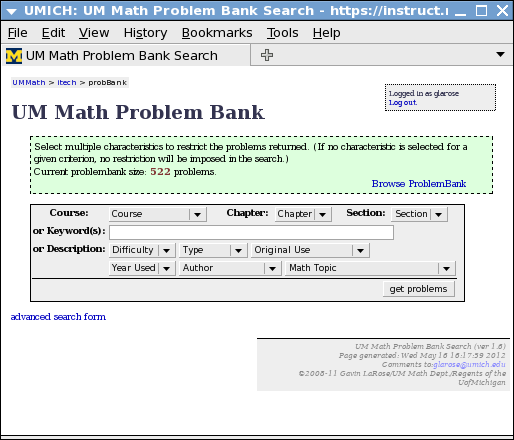
\includegraphics[height=2.5in]{um_search1}\quad
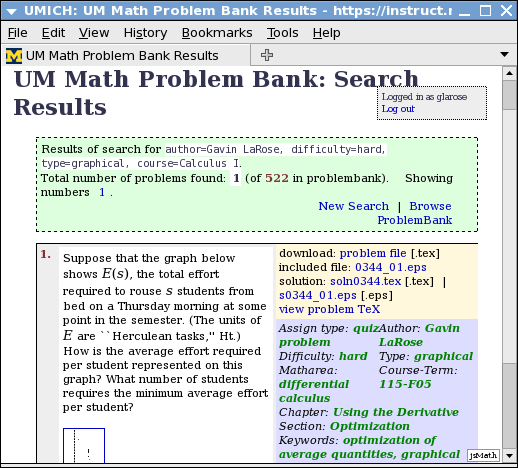
\includegraphics[height=2.5in]{um_result1}\\
\caption{UM Problem Library: left, search form; right, sample search result}
\label{umprobbank}
\end{center}
\end{figure}

The problem library in use in the mathematics department at the University
of Michigan is shown in Figure~\ref{umprobbank}, which shows the
search interface and a sample problem as displayed in a search result.
This illustrates in a general way the basic search characteristics that
will be supported by ROPE: the ability to locate problems that are
associated with specific topics in a course, which are of varying levels
of difficulty, that have specific characteristics (such as use of
graphically presented or tabular data), or which were used in specific
contexts (as homework problems, on quizzes, etc.).  This project will
dramatically rework this application, allowing it to address the goals
that are laid out in the introduction of this proposal, by including
\begin{itemize}
  \item
    scalability to support many more users, problems and problem formats,
  \item 
    community site membership and interactions,
  \item 
    problem moderation and editing,
  \item 
    problem filtering to generate alternate formats from existing
    formats,
  \item
    a modern, flexible interface that supports these features, and
  \item
    a well-documented API that will allow other applications to
    communicate with ROPE in manners other than through the browser
    interface.
\end{itemize}
These goals are described in greater detail in the following subsections.

\begin{subsection}{Scalability}

The problem library at the University of Michigan runs behind the
University web-login system and has access restricted to instructors in
the mathematics department. It accordingly supports a user base of several
hundred users, all of whom are defined by external data sources and need
no further identification or system characteristics. ROPE will support
thousands of users with internally defined characteristics (names, e-mail
addresses, password information, etc.). Accordingly, we will in the course
of the project expand the database used for the University of Michigan
system to support this. In addition, we will establish the workflow to
allow for users to author, submit and rate problems, determine the
appropriate manner in which moderation, editing of and commenting on
problems should take place, and add these functions to the problem code.

Problem types supported by the University of Michigan problem bank are
\LaTeX\ and external formats (\emph{Word} or \emph{OpenOffice} document
snippets). All problems for the problem bank are currently maintained as
separate files. For ROPE we will completely revise the problem data
structures so that all problem data are maintained in the system's
database, and completely rework the data maintained for problems to extend
the types of descriptive data for the problems and to support additional
file formats and the ability to add additional formats as they become
useful.

\end{subsection}

\begin{subsection}{Community and Site Moderation}

An aspect that is missing from the current problem bank is a mechanism for
users to provide feedback on the quality and usefulness of problems. ROPE will address this by including the ability for users to vote and
comment on problems in the library.  The data management and manner in
which this is to be done will be added to the current problembank
model.  In addition, problem view/download statistics will be provided as
part of the metadata about problems.

We will determine the nature of the voting/commenting system used, in
consultation with the Advisory Group, with the goal of maximizing its
usefulness and minimizing the possibility of any abuse. ROPE will also
support comment and problem flagging so that problems or comments with
errors can be updated by ROPE moderators. We anticipate that the moderators
will initially be drawn from the grant personnel, and will work with the
Advisory Group to determine the best manner to expand the group of people
who are engaged in this activity.  (We discuss the project's Advisory
Group in the following sections.)  ROPE will also support problem
authoring or submission from users in its community.  The degree of
moderation for this activity (if any) will also be determined by the
project personnel, including our Advisory Group.

In addition, ROPE will support a sharable problem collection feature.
This will allow users to create problem lists for their own
uses---homework sets for given courses, etc.---and to share these lists.
Thus an instructor teaching a course will be able to share her/his problem
lists with other faculty at her/his institution, or with colleagues at
other institutions.  In addition, book authors (and publishers) could
build problem lists for their texts that would then be openly available
for anyone using those texts.

\end{subsection}

\begin{subsection}{Problem Filtering}

As we add additional problem formats to ROPE, we will build in the
ability to convert between some of the formats and output types, and to
add additional filters as they are needed and developed. We anticipate
three initial filters:
\begin{itemize}
  \item
    a filter converting \TeX\ formatted problems to PDF output;
  \item
    a filter converting \TeX\ formatted problems to a rudimentary WeBWorK
    problem file; and
  \item
    a filter converting WeBWorK formatted problems to \TeX\ output. 
\end{itemize}
These will serve to provide significant additional functionality to ROPE and will be templates that illustrate the manner in which additional
filters may be constructed.

\end{subsection}

\begin{subsection}{Interface}

Considering these features and goals, it is clear that the simple search
and results interface used by the University of Michigan problem bank
system (Figure~\ref{umprobbank}) will need to be completely re-imagined.
We, with our Advisory Group, will work to develop an entirely new
interface that supports the precision of searching that we need and the
multitude of new data and features that ROPE will support.

\end{subsection}

\begin{subsection}{API and Documentation}

A natural extension to the filtering system that will be developed for ROPE is a mechanism by which other applications can use the generated
problem formats. To allow this, we will develop an easily used API by
which external applications may query ROPE to get file or problem data
for specified problems. A first application for this will be to allow the
open-source web homework system WeBWorK to include problems drawn from ROPE.  We will work with WeBWorK developers and the WeBWorK leadership
group on this aspect of the project.

\end{subsection}

\end{section}

\begin{section}{Project Implementation and Timeline}

To implement ROPE, as described in the preceding section, we have the
timeline laid out in Figure~\ref{timeline}.  This illustrates the four
phases in which we expect work on ROPE to be carried out.  The first,
to be completed by the end of the spring semester of 2015, is a \emph{Data
and Interface Design} phase.  In this time we, in consultation with
the Advisory Group, will determine the requirements for the database
supporting ROPE and lay out its on-line user interface.

\begin{figure}
\begin{center}
\begin{tabular}{|l|l|l|l|}
  \hline
  \textbf{date} & \textbf{personnel} & \textbf{activity} & \textbf{outcome}\\
  \hline
  \hline
  January 15 & PMs & team meeting (JMM) & initial design and data proposal\\
  \hline
  Spring 15 & AG, PMs & on-site meeting
	& feedback on design and data proposal\\
	& PMs & on-line meetings & finalize design and data models\\
  \hline
  Summer 15 & PM, Pr & programming work & database, alpha
	software developed \\ 
	& PMs & library development & initial library population \\
	& PMs, EE & on-site meeting & initial evaluation \\
  \hline
  Fall 15, & PM & programming work & user interface finished (if
	necessary) \\ 
  Spring 16 & PMs & library development & expansion of library population \\
	& PMs, At & initial testing & alpha testing of ROPE \\
  \hline 
  January 16 & PMs & team meeting (JMM) & evaluation of alpha software,
	initial library \\
  \hline
  Spring 16 & PMs & on-site team meeting & filter \& API data proposal \\
  \hline
  Summer 16 & AG, PMs & on-site meeting &
 	feedback on filters \& API, alpha test \\
	& & & finalize model for moderation \\
	& PMs & on-line meetings & finalize filter \& API ruleset \\
	& PM, Pr & programming work & debug alpha software \\
	& & & implement filtering and API \\
  \hline
  Fall 16 & PMs, Bt & beta testing & beta use of ROPE \\
	& PMs, EE & on-site meeting & second evaluation \\
  \hline
  January 17 & PMs & team meeting (JMM) & evaluation and planning \\
  \hline
  Spring 17 & PMs & dissemination & continued beta use of ROPE \\
  \hline
  Summer 17 & PM & programming work & debugging, updates beta to
	production \\ 
	& PMs & editorial work & documentation completed \\
  \hline
  Fall 17, & PMs & programming work & production service debugging\\
  Spring 18 & & editorial work & documentation updated \\ 
  \hline
\end{tabular}
\caption{Project Timeline: personnel notation---PMs = grant project
  managers (Ernst, Hamblen, LaRose); AG =
  Advisory Group; Pr = contract programmer; EE = External Evaluator; At =
  Alpha testers; Bt = Beta testers}
\label{timeline}
\end{center}
\end{figure}

The second phase of work, \emph{Alpha Product Development} will be carried
out in the summer of 2015 and, as necessary, fall of 2015.  In this phase
Gavin LaRose will work with the hired programming consultant to develop
the database and software required for the initial version of ROPE.
Dana Ernst and Spencer Hamblen will develop problems for, and recruit
alpha-testers to use, this initial version, which we will launch in the
fall of 2015.  A key part of our alpha testing will be recruitment of 15
alpha testing consultants.  These will be users who will be paid a small
honorarium to encourage their use of ROPE, and their contributions to
the library.  These users will be contacted regularly in the course of the
fall and spring semesters to get their feedback on aspects of the system
which need revision as well as on those components which are working well.

In the third phase of the project, \emph{Extensions and Beta Development},
taking place in spring and summer 2016, we will develop the technical
requirements for the problem filtering supported by ROPE and the API by
which other applications may interact with it.  In the spring and summer
we will finalize these requirements with the Advisory Group, and in the
summer Gavin LaRose will work with the programmer consultant to implement
these features.  Also in the summer Dana Ernst and Spencer Hamblen will
continue to expand ROPE and recruit additional beta testing
consultants.  These users will serve in a similar role to the alpha
testing consultants.

The final phase of the project will see it move from beta to a
\emph{Production Service}.  This phase will take place in summer and fall
of 2017.  There are three components of this: finishing debugging and
updates that were suggested by the beta testing, moving the service to
production hardware, and completing documentation and dissemination.  The
first two phases of these will be completed by Gavin LaRose, in
conjunction with the systems support staff at the University of Michigan's
mathematics department.  The remaining tasks will be accomplished by all
project managers, with Dana Ernst and Spencer Hamblen taking the lead.

Finally, the Math Department at the University of Michigan will be able to
provide the required technical support to initially implement and
subsequently maintain the computer hardware required for this project.
While it is in development and alpha and beta testing ROPE will be
hosted on webservers that are currently maintained in the Department and
which have the required server capacity to support the project.  As the
project is transformed to a production service we will move it onto its
own server, purchased using grant money, which will be housed and
supported in the Department.

\end{section}

\begin{section}{Project Personnel}

The grant will be managed by Gavin LaRose, University of Michigan, Dana
Ernst, Northern Arizona University and Spencer Hamblen, McDaniel College.
Stephen DeBacker, University of Michigan, will oversee the project as it
is implemented at the University of Michigan.  Their expertise position
them well to successfully carry out this project.

\textbf{Gavin LaRose} is a lecturer~IV and manager of instructional
technology in the Department of Mathematics at the University of Michigan.
His research interests are in applied mathematics, specifically biological
modeling, but he has for the majority of his time post-Ph.D. been
primarily focused on undergraduate education.  He has been a developer for
the WeBWorK open-source homework system and wrote the majority of the
testing module for that system.  In his role in instructional technology
at the University of Michigan he has created a wide range of on-line
applications in use at the University of Michigan, including data
management and tutorial systems.  He is the author of the problem library
that is currently in use at the University of Michigan, which will serve
as the early prototype for ROPE.  He has won several teaching awards,
most recently the University of Michigan College of Literature, Sciences
and the Arts \emph{Matthews Underclass Teaching Award} and the Michigan
MAA Section's teaching award.

\textbf{Stephen DeBacker} is an \emph{Arthur F. Thurnau} professor of
mathematics in the Department of Mathematics at the University of
Michigan, a named chair designation given to tenured faculty whose
commitment to and investment in undergraduate teaching has had a
demonstrable impact on the intellectual development and lives of their
students.  His research interests are in questions in harmonic analysis
for reductive p-adic groups, and specifically in stability questions.  As
the Director of Undergraduate Programs in the mathematics department, he
oversees the department's major and non-majors courses and content,
advising of majors, and significant educational initiatives in the
department.  He will work with Gavin LaRose to oversee the project as it
is implemented at the University of Michigan.

\textbf{Dana Ernst} recently completed his fourth year as an assistant
professor at Plymouth State University in Plymouth, NH.  However, in the
fall of 2012, he will begin working at Northern Arizona University, where
one of his main service duties will be to revamp the calculus sequence to
include more inquiry-based pedagogy.  Ernst's primary research interests
are in the interplay between combinatorics and algebraic structures.
Ernst is also passionate about undergraduate mathematics education and
recently his research interests have included topics in this area. In
particular, he is studying the effectiveness of a collaborative approach
to inquiry-based learning.  Furthermore, he is interested in the use of
technology to aid in the learning of mathematics and would like to study
its impact on student success.  In addition to using free and open-source
software (such as \emph{Sage}), Ernst is inspired by the recent
open-content textbook movement and strongly believes that educators should
choose free, open-source, or low cost textbooks when viable alternatives
exist.  Ernst has been the recipient of several teaching awards, most
recently being named the 2009 and the 2011 \emph{Plymouth State University
Distinguished Mathematics Professor}, an honor determined by the math
majors at Plymouth State University.  Moreover, he was recently a
finalist, and PSU's sole nominee, for the statewide \emph{New Hampshire
Excellence in Education Award}.

\textbf{Spencer Hamblen} is an Associate Professor at McDaniel College in
Westminster, MD.  His main research interest is Galois representations and
deformation theory, but has recently been working in arithmetic dynamics
and leading student research on classical arithmetic functions and problems 
in elementary number theory.  His interest in the ways problems shape 
students' view of mathematics began while a graduate student at Cornell 
working with the GoodQuestions project.  This interest has continued in his 
current teaching of courses that rely heavily on student problem-solving 
and other inquiry-based learning courses.

The Advisory Group for the grant represents constituencies that will have
particular interest in ROPE, and includes individuals with a wide range
of backgrounds and experience that will allow them to provide insight and
advice on the project.  \textbf{Robert Beezer} is professor of mathematics
at the University of Puget Sound.  He is an open-content textbook author,
having authored a linear algebra textbook, and is an advocate for
open-content authoring who has worked with other textbook authors.  He is
also involved in the Sage open-source mathematics software system.
\textbf{Matt Boelkins} is associate professor of mathematics at Grand
Valley State University and is currently developing an open-content
calculus textbook.  \textbf{Michael Dorff} is associate professor of
mathematics at Brigham Young University.  He is the director of the
NSF-funded BYU summer mathematics REU and the director of the NSF-funded
Center for Undergraduate Research in Mathematics (CURM).  \textbf{Steve
Dunbar} is professor of mathematics at the University of Nebraska,
Lincoln, and is the MAA's Director of Competitions.  He has made some
initial steps toward coding problems from the American Mathematics
Competitions, which he directs, to make them useful for other
applications.  \textbf{Kathi Fletcher} is a Shuttleworth Foundation Fellow
working on the development of open educational resources and has a
background in computer science.  She is working to accelerate both the
production of high-quality, reusable Open Educational Resources (OER) and
the development of innovative learning environments that build upon OER.
\textbf{Jeff Holt} is professor of mathematics at the University of
Virginia, and is one of the authors and continued developers of the
WeBWorK national problem library.  \textbf{Aaron Wangberg} is associate
professor at Winona State University.  His group has written whiteboard
and adaptive homework tools which utilize WeBWorK and the National Problem
Library to conduct mathematics education research.  His group leads the
discussion with the Research in Undergraduate Mathematics Education
community on how to conduct and disseminate research programs using an
open framework.

All of the members of the advisory group have expressed enthusiasm for the ROPE project and willingness to serve in this capacity.

The project will have an external evaluator, \textbf{Doug Ensley}, who
will meet on-site twice in the course of the project to provide formative
feedback.  Doug Ensley is professor of mathematics at Shippensburg
University, has been editor of the Mathematical Sciences Digital Library,
has written a discrete mathematics textbook, and is currently second vice
president of the MAA.  He has written a library of computer based material
for the teaching and learning of mathematics and has written award winning
Adobe Flash educational materials.

In addition to these individuals, we will hire a programmer to assist with
the coding and database revision that will be done to the University of
Michigan codebase in the course of developing ROPE. These revisions
will be significant, and the programmer will work in close collaboration
with Gavin LaRose to develop a codebase for ROPE which will then be
open and easily maintained and extended as appropriate. 

\end{section}

\begin{section}{Intellectual Merit}

ROPE project will address a current need in undergraduate mathematics
education: the need for a widely available source of good problems that
instructors can use in a variety of educational venues.  Much of the
learning that takes place in mathematics, and other STEM fields, is driven
by students' work, and the success of that learning is fundamentally
dependent on the types of problems on which they work.  We therefore
expect ROPE to have the potential to be a significant and widely used
tool to enhance student learning.  

There are several specific aspects of ROPE which will have direct
bearing on this.
\begin{itemize}
  \item
    Its on-line search page that allows precise searches for specific
    types of problems.
  \item
    The open nature of the system that allows a wide range of uses of the
    problems in the library.
  \item
    The user feedback and statistics available for the problems in the
    library. 
  \item
    Users' ability to create their own problem sets, and to share
    these with other users.
  \item
    The explicitly extensible design of the system, allowing multiple
    problem formats and conversions between them.
\end{itemize}

Taking these together, we expect that ROPE will develop into an
easy-to-use, widely adopted resource with a correspondingly significant
impact on student learning of undergraduate mathematics.

\end{section}

\begin{section}{Broader Impacts}

The broad impact of ROPE will stem from its accessibility, ease-of-use
and extensibility.  We believe that the features that we are including in
ROPE will result in its use by many faculty at many institutions.  We
expect that the largest group of users of ROPE will be faculty who are
browsing for additional homework, test or quiz problems for their courses.
Even with a well-written textbook there are routine and inevitable cases
in an instructor will be at a loss to find a problem that s/he likes, and
ROPE will be the perfect resource to fill that gap.  In addition, as
open-content textbooks expand in popularity and availability, the
usefulness of ROPE will similarly increase.  We anticipate that
textbook authors may choose to define problem sets in ROPE for use by
instructors using their texts whether they are publishing open-content
textbooks or working with a publisher (though it is clear that the
attractiveness of ROPE to the former may be significantly greater).
And because ROPE will be designed from the outset to be flexible and
extensible, it will be able to meet the changing needs of faculty in the
future and make connections with other software projects for which a
library of open problems will be useful.

All told, we expect that ROPE should have very broad impact, reaching
instructors at all types of colleges and universities who are teaching any
standard mathematics course in any of a number of different ways.  We
further expect that as ROPE develops we will be able to extend it to
include other disciplines, also increasing its impact.

\end{section}

\begin{section}{Dissemination}

Key to the success of ROPE will be its dissemination: for it to be able
to reach and help many instructors, they must know of its existence.  To
successfully ensure that mathematics faculty are aware of ROPE, we will
pursue a four-fold dissemination plan: generating a primary user base by
soliciting and engaging likely users, publicizing the availability of ROPE to the networks of colleagues available to the Ernst, Hamblen and
LaRose, publicizing ROPE to the larger community, and communicating
with professional organizations and open-source projects to make
connections with their members.

To generate a primary user base for ROPE, we will actively solicit
alpha and beta testing consultants of ROPE.  These users (about 15
individuals for each of the alpha and beta development phases of the
project) will be selected by Ernst, Hamblen and LaRose (in consultation
with the Advisory Group) as people we expect will have interest in ROPE, and whose role with the project is likely to be more than simply
searching for problems.  We will encourage their participation in rating
problems, making comments and providing problem groups, by offering them a
small honorarium for their work.  Having these individuals will provide a
critical mass of actively engaged users of ROPE in the critical phases
of its development, which will help develop its user-base in the long
term.

The personnel managing this project are well-positioned to communicate
with a large number of faculty who are likely to be users of ROPE
because of their connections with other projects and organizations.  All
three of the Ernst, Hamblen and LaRose are Project NExT [2]
%\cite{projectnext}
Fellows, and Gavin LaRose is a member of the Project NExT leadership team.
Project NExT is a professional development program of the MAA which
supports new math faculty in all aspects of their professional career,
with an emphasis on teaching.  There are over 1300 Fellows from all parts
of the United States and some surrounding countries and territories, and
they are distinguished by their energetic embrace of new ideas and
effective teaching strategies.  We will publicize ROPE to the Project
NExT Fellows, and have good reason to expect that many of them will become
significant users of ROPE.  In addition, the mathematics department at
the University of Michigan provides a large potential base of users not
only at the University but at other institutions as well.  Each academic
year, approximately 150 graduate students, post-doctoral and regular
faculty teach in its Introductory Program courses, and we will publicize
the availability of ROPE to them.  The majority of these graduate
students and post-docs go on to take other academic positions, and will
take their use of ROPE with them to those positions.

To promote awareness of ROPE among individuals and groups with whom we
and the Advisory Group do not have personal contact, we will disseminate
information about ROPE at national mathematics meetings.  This
dissemination will include presentations in poster and contributed
sessions at the MAA's MathFest in the summer and the Joint Mathematics
Meetings (JMM) in the winter, which attract essentially all potential
users of ROPE (though we suspect they may not all choose to come to our
presentations).  At the JMM we will also rent a booth in the exhibit hall
for the meeting to have a demonstration of ROPE.  Because the exhibits
are a popular attraction of the JMM, we expect this will increase the
number of people who are aware of ROPE by several hundred.  In
addition, we will disseminate fliers about ROPE at the booth and in
person at the meetings.

Finally, we will work with professional organizations and the larger
open-source communities to promote ROPE.  The project personnel are
involved with many communities with whom we will make contact, including
the MAA, WeBWorK and Sage, and we will work to develop additional contacts
and communication channels with these groups.

\end{section}

\begin{section}{Evaluation}

The success of ROPE will be measured by a number of quantitative,
measurable outcomes that will assess the degree to which it has been
adopted by the mathematics community, and by a number of more qualitative
measures that seek to discern its impact on student learning.  Both of
these will be adjusted and expanded in consultation with our external
evaluator.  As indicated in the project timeline, our first consultation
with the evaluator will be early in the project development, in the summer
of 2015.  This early meeting will allow us to work with the evaluator to
determine if the outcomes that we have set forth are appropriate, revise
the goals that we have for our measurable outcomes, and determine areas in
which our evaluation plan may be improved.  The second visit will be just
past the midpoint of the project, in fall 2016, to provide us with an
objective assessment of the manner in which the evaluation plan has been
put into place and what it can tell us.  At that time the evaluator will
also work with us to arrive at an updated plan that can be carried forward
to provide a long-term and sustainable evaluation cycle for the project.

Our primary measurable outcomes have to do with the scope of the library
and its number of users.  Because the usefulness of ROPE will be driven
by the number of problems it provides, this will be our first measure of
success; in tandem with this, we will consider the number of courses for
which there are a reasonable number of problems.  For the purposes of our
evaluation, we consider a reasonable number to be that which we feel would
likely allow a user to populate homework assignments for the
course---about 200 problems.  Given the resource, however, the next
measurable objective is to have a significant base of users who are using
the problems in ROPE, authoring and submitting additional problems, and
providing feedback on the problems.  To judge users' engagement with ROPE, we will use as measures the number of users who register with the
site, the number who are providing feedback on problems, the number of
problem collections users have defined in the system, and the number of
users who have contributed at least five problems to the library.  In
Figure~\ref{outcomes} we summarize these measures and our goals for them
over the course of the project.

\begin{figure}
\begin{center}
\begin{tabular}{|l|l|l|}
  \hline
  \textbf{Outcome} & \textbf{Goal for summer '16} & \textbf{Goal for
  Summer '17} \\
  \hline
  \hline
%%   \# of hits & ? & ? \\
%%   \hline
  \# of supported courses & 6 & 15 \\
  \hline
  \# of problems & 2000 & 5000 \\
  \hline
  \# of registered users & 200 & 1000 \\
  \hline
  \# of users who submitted rating data & 50 & 150 \\
  \hline
  \# of problem collections & 50 & 200 \\
  \hline
  \# of problem authors & 30 & 75 \\
  \hline
  \# of institutions using & 15 & 40 \\
  \hline
\end{tabular}
\caption{Primary Measurable Outcomes and Goals}
\label{outcomes}
\end{center}
\end{figure}

Measuring the impact of ROPE on student learning is an exceedingly
formidable problem.  We are therefore forced to consider indirect measures
that may suggest the quality of the resource which we are providing and
its impact.  The two primary measures that we will use for this are the
ratings and comments on the problems in ROPE and the number of students
and courses using problems from ROPE.  We have some faith in the
ability of instructors to reasonably evaluate the usefulness and quality
of problems that they assign in their courses.  Because of this, we will
use the ratings they give to problems and comments that they have about
the problems in ROPE as an indirect measure of the quality of the
problem library.  Our measurable outcome for this goal is that 20\% of the
problems in ROPE will have been marked as ``liked'' by at least 2\% of
the registered number of users.  A second indirect measure of impact is to
determine how many students are in classes using ROPE.  We will assess
this through the end of our alpha testing (that is, when the number of
users is small enough for us to be able to do this).  We will contact our
alpha testing consultants to determine the number of problems they are
using, the number of courses they are using the problems for, and the
number of students in those courses.  From these users our goal is to have
300 students using at least 20 problems from ROPE by the summer of
2016. 

\end{section}

\end{document}

\begin{thebibliography}{9}

\bibitem{mathquest} Cline, Kelly, Mark Parker and Holly Zullo.
    ``MathQUEST/MathVote.'' On-line resource. 2012.  Carroll College.
    accessed 5/17/12.
    \texttt{<http://mathquest.carroll.edu/>}.

\bibitem{projectnext} Higgins, Aparna, Joe Gallian, Judith Covington, and 
    Gavin LaRose.  ``Project NExT.''  On-line information.  2012.
    accessed 5/17/12.
    \texttt{<http://archives.math.utk.edu/projnext/>}.

\bibitem{webwork} The Mathematical Association of America.  ``WeBWorK.''
    Website.  2012.  accessed 5/17/12.
    \texttt{<http://webwork.maa.org/>}.

\bibitem{quadbase} Rice University.  ``Quadbase.''  On-line resource.
    Unknown authoring date.  accessed 5/17/12.
    \texttt{<http://quadbase.org/>}.

\bibitem{goodquestions} Terrell, Maria, Robert Connelly, David Henderson,
    and Robert Strichartz.  ``The GoodQuestions Project.''  On-line
    resource.  2005. Department of Mathematics, Cornell College.  accessed
    5/17/12.
    \texttt{<http://www.math.cornell.edu/$\sim$GoodQuestions/>}.

% http://imathas.com/index.html ?

\end{thebibliography}

\end{document}



